% Tulokset / results
\section{Experiments}

% is X? test X. proof: X is ?.

\subsection{Synchronization issues}

Synchronizing the image sources temporally is important for reconstruction algorithms to work correctly.
A synchronized system captures images from all cameras with a reasonably small time difference, so that subject movement does not introduce additional errors.

\subsubsection{Shutter delay} \label{sec:shutterdelaymeas}

Shutter delay consistency among cameras and shots blah blah.

An input pin of the MCU was connected to the hot shoe flash present in the camera body.
Assuming a negligible delay between the flash trigger signal and the actual photo exposure, the time between shutter button and signal from the flash connector is the shutter delay.
The camera was set up to all manual settings and manual focus.
Measurements matched consistently the 75 millisecond delay found in various sources, repeated shots varying less than a millisecond.
This suggests that even fast moving subjects can be captured properly.

\subsubsection{Still capture}

Static subjects do not move or change shape.
However, still imagery of e.g. a human head needs at least semi-accurate syncing, because standing still enough is not possible for longer periods (seconds).
Even though the facial pose would not change, the wrong position of the head in a frame would introduce error.
Similarly, capturing e.g. a still image of a moving cloth needs proper synchronization.

For a completely static subject, the cameras can even be shot separately, each using its own integrated flash unit, to minimize shadows for each viewpoint.
When the light direction is almost the same as the camera's view direction, no shadows are possible.

Still capture using the wired remote trigger was analyzed with a moving object.
A standard 120 mm PC fan was rotated in the view of all cameras, with markings drawn around the fan and in the moving blades with a bright-colored pen.
The cameras were set to maximum aperture (f/1.8) and shortest possible shutter speed (1/4000 s) to minimize motion blur.
The fan speed had to be reduced by using 4.5 volts instead of the nominal 12 volts, resulting in about TODO revolutions per second, or TODO m/s on the far end of the fan blades.

Without any actual measurements done but only with careful manual observation, no significant sync mismatches were found by comparing the position of the rotating measurements in all nine different images.
Two such images are depicted in figure \ref{fig:fansynctest}.

\simplefig{h}{%
%\setlength\fboxsep{0pt}
%\setlength\fboxrule{1pt}
%\fbox{
\includegraphics[width=0.3\textwidth]{flashtiming-a}}
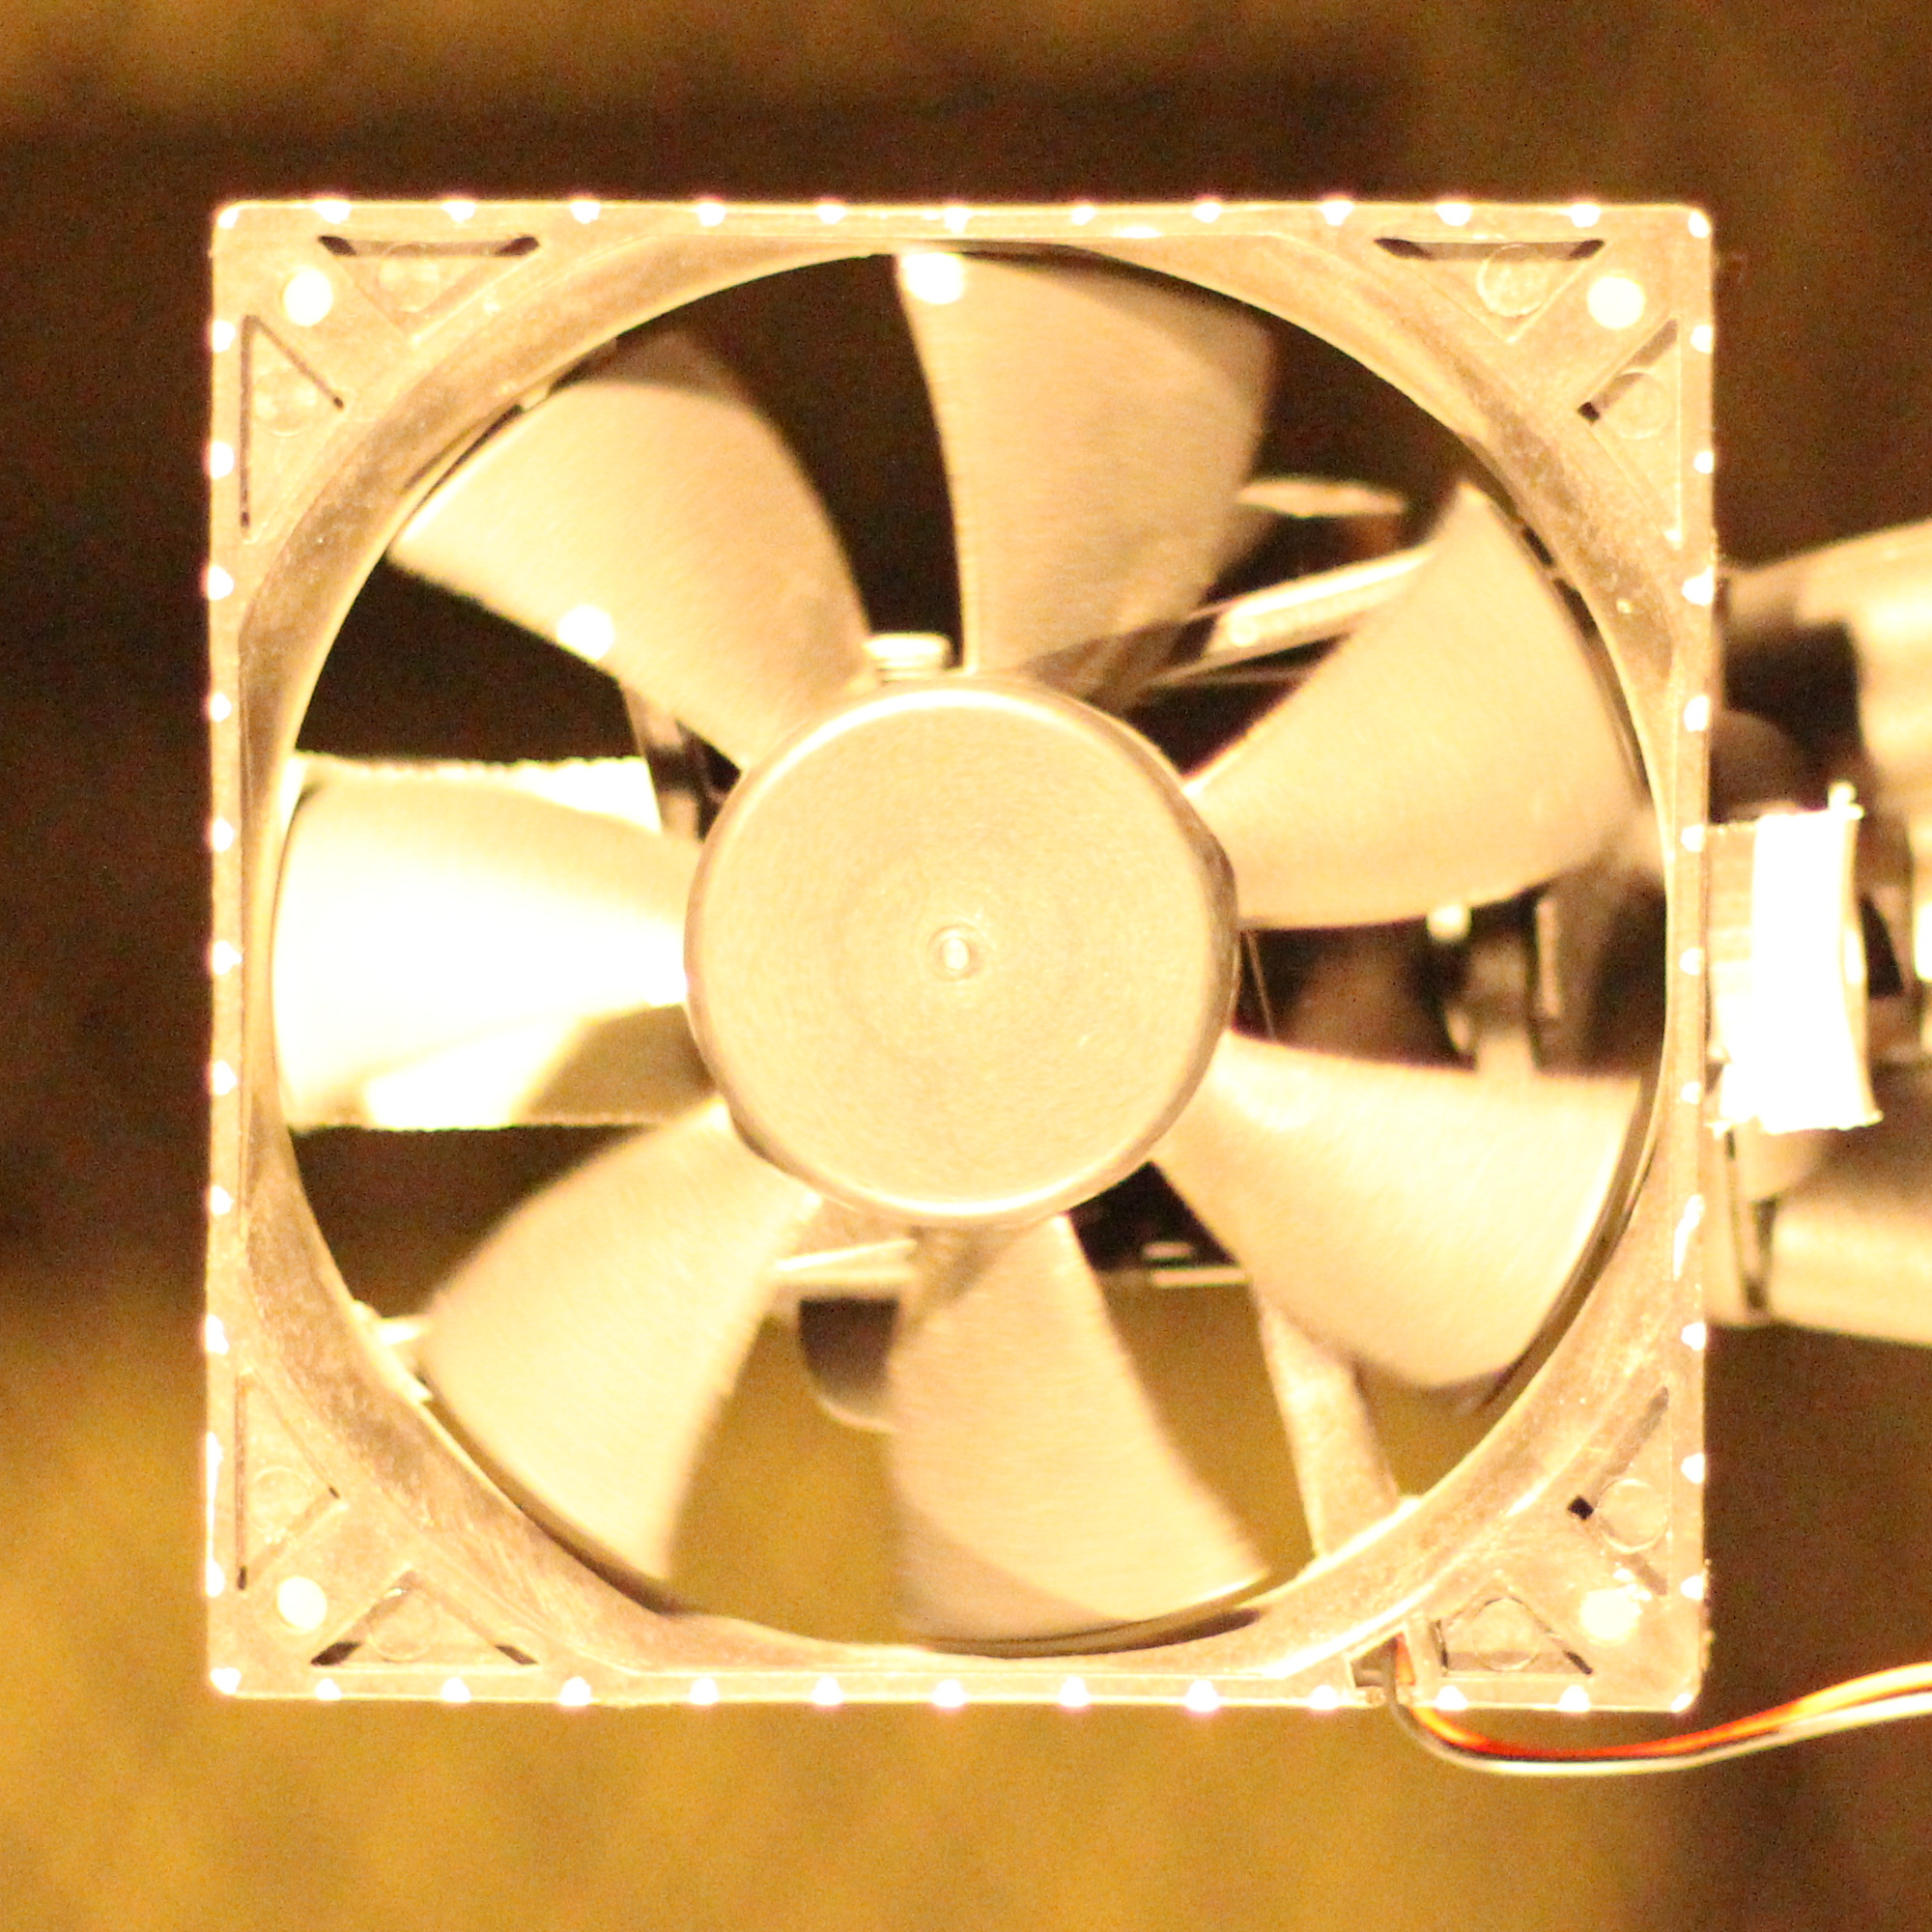
\includegraphics[width=0.45\textwidth]{fan-a}
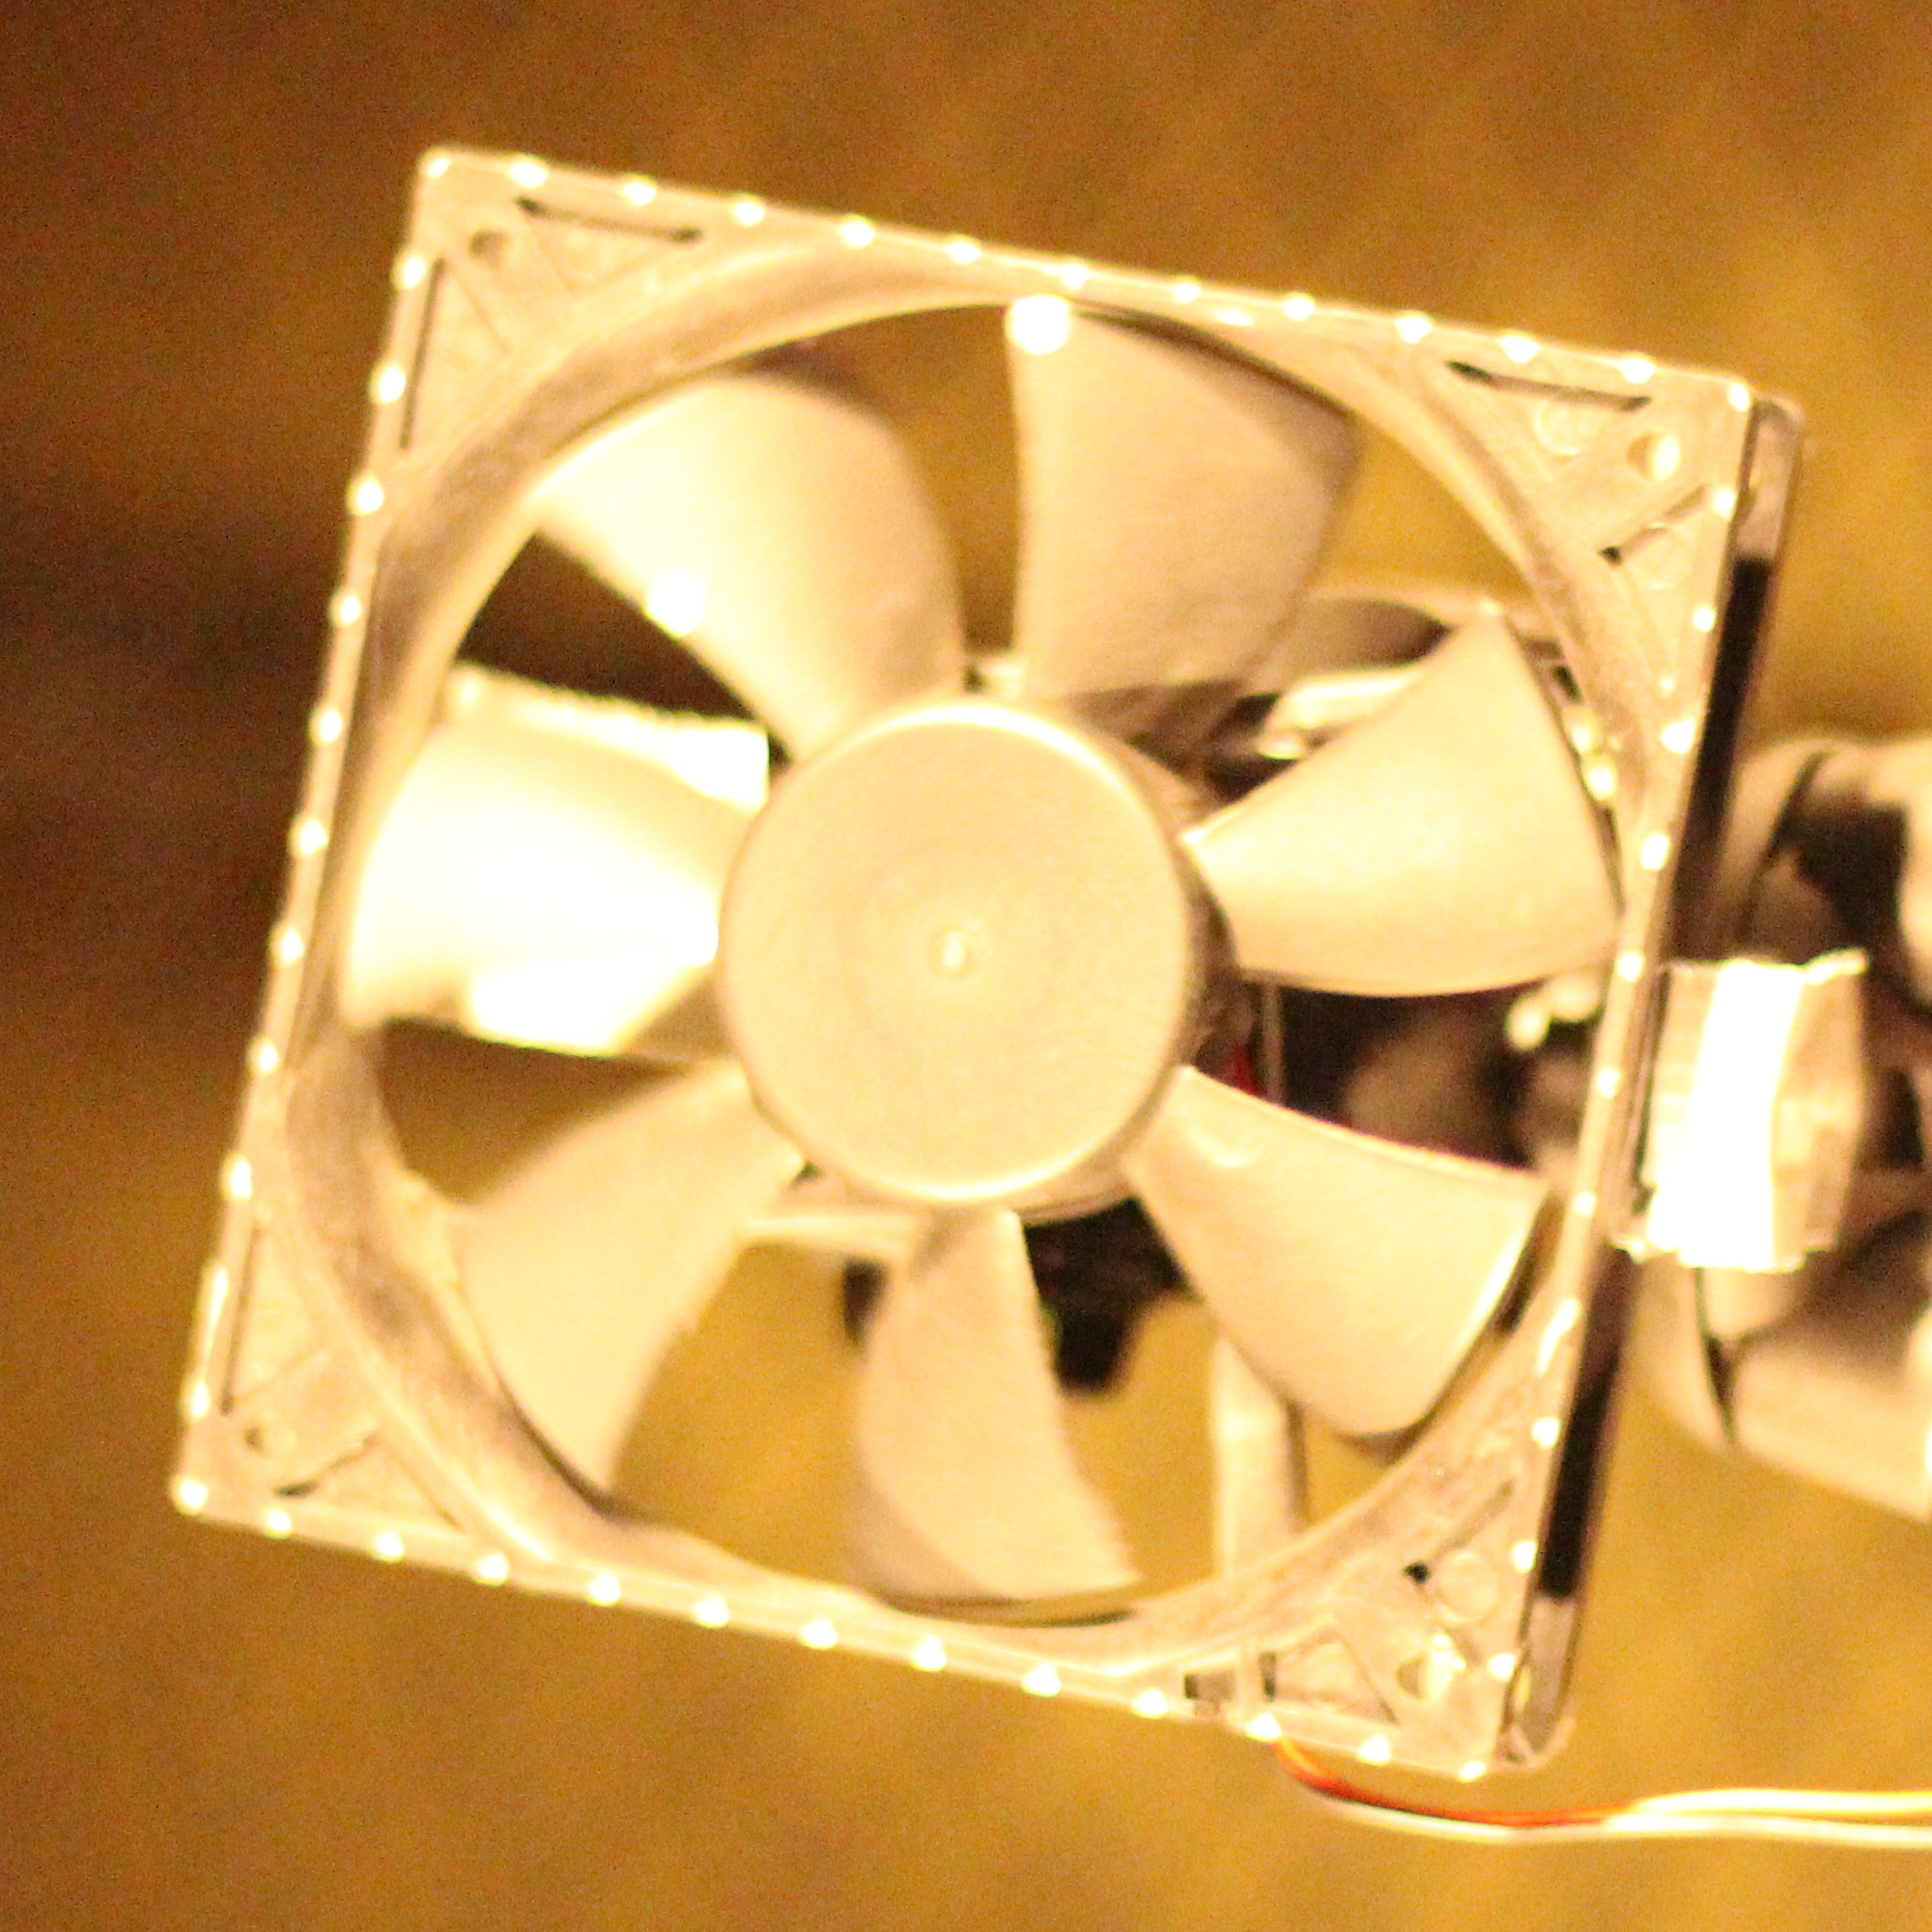
\includegraphics[width=0.45\textwidth]{fan-b}
}{fig:fansynctest}{
	Frames from two cameras in a synchronization test with a PC fan. A marking on the end of a fan blade can be seen in the top.
	The position of the marking does not differ distinctively in the pictures.
}

% TODO: testaa kans huomaako jos vaikka yksi ei oo synkassa
% "hardly scientific" jonnekin väliin, hehheh?
%Another test was done using a mobile phone microphone.
%A DSLR makes a distinct clanking sound because of its mirror and mechanical shutter.
%Two sound clips were recorded several times: the sound of all cameras triggering at the same time, and for comparison, the sound of a single camera only.
%The waveforms were drawn on top of each other and inspected, and no distinct difference was found.
%For comparison, also intentionally wrongly synchronized sequences were recorded.
%
%\simplegfx{p}{0.8\textwidth}{shutteraudio}{
%	Trimmed audio recordings of all cameras shooting (top), and only a single camera (bottom).
%	The waveforms cannot be clearly distinguished.
%}


\subsubsection{Video capture}

% intro

The EOS 700D does not support an external sync signal for video recording, but relies on an internal clock to sync the frames within a single video file.
It can be safely assumed that the clock speed has little variation, and thus, little drift and jitter occur in the videos.
Recording offset remains an issue;
processing time of each camera from the shutter button to start of first frame varies because of unknown reasons; even though a wireless remote control of the camera manufacturer would be used for starting several cameras at once, the offset is very noticeable.

% what was done

A test was carried out to find variations in the recording offset.
Three cameras were triggered with a Canon RC-6 wireless remote control.
The remote sends a short infrared pulse to a sensor in the front of a camera when a key is pressed.
The camera was set in video mode and it was configured to use the remote release.
%The exposure time was set to minimum, 1/4000 s, to maximise the rolling shutter effect.
%In this mode, the sensor rows are exposed one by one in succession.
When all cameras were recording, a flash unit (Canon Speedlite 420EX) was aimed at the lenses and fired manually several times.

% what happens

A direct light pulse of a flash unit shows up as an over-exposed, completely white video frame, if the whole frame was exposing the image during the light pulse.
Sometimes only part of the frame would be exposed to the flash light as a rolling shutter effect.
Because the CMOS sensor is cleared and read line by line, the time of the flash can be deduced from the first bright line in the image.
The rows are zeroed from light in succession in the same way as a mechanical focal plane shutter moves and exposed until read.
Thus, the flash light's starting time in the video's internal clock is the frame's start time plus the duration that it takes for the rows before the overexposed one to show up:

\begin{align} \label{timingcalib}
t_{Cl} &= t_{Ci} + t_{Cf} \\
&= i_C * F + f_C / R * F \\
&= (i_C + f_C / r * c) * F
\end{align}

where $C$ is a camera identifier, $t_{Cl}$ is camera-relative time for the light pulse, $t_{Ci}$ is the starting time for the frame where the light shows up, and $t_{Cf}$ is the time inside the particular frame.
The frame index $i$ marks the number of the frame in the video file, starts from 0, and there is $F$ = $1/\text{fps}$ time between the frames.
$f_C$ is the first exposed row, $R = r / c$ is the time for a single row to expose, $r$ is the vertical frame resolution and $c$ is a correction coefficient describing the relation of exposure time and frame duration ($0.5$ in this case, referring to 180 degree shutter).
Offset between two cameras $A$ and $B$ is then $t_{Al} - t_{Bl}$.
The timings are depicted in figure \ref{fig:flashtimeline} as a timeline with matching symbols.

For perfectly synchronized videos, the frames would be identical, and time difference calculated with eq. \ref{timingcalib} for each frame would be zero as $i_C$ and $f_C$ would be constants for all $C$.
A typical measurement result is shown in figure \ref{fig:flashtiming}.
Audio recorded by the cameras' internal microphones at the same event is shown in figure \ref{fig:flashaudio}, and the order of flash pulses in the three frames can be verified from the order of the sound emitted by the flash.

\simplegfx{h}{1.0\textwidth}{flashtimeline}
{Illustration on timing calibration of two cameras using a flash light.
The darkened areas represent the exposure times and the red band represents the light pulse.
In this example, $c = 0.5$.
}

\simplefig{p}{%
\setlength\fboxsep{0pt}
\setlength\fboxrule{1pt}
\fbox{
\includegraphics[width=0.3\textwidth]{flashtiming-a}}
\fbox{
\includegraphics[width=0.3\textwidth]{flashtiming-b}}
\fbox{
\includegraphics[width=0.3\textwidth]{flashtiming-c}}
}{fig:flashtiming}
{Video frames of three cameras started with the same remote, with the same frame index.
The time for the flash unit to reach maximum brightness is almost instant.
The start of the light pulse can be seen in the leftmost and rightmost frames.
In the middle one, the flash has been fired before the frame exposure started;
the frame before it is still without any overexposed light.
It is impossible to deduce the exact time in this case.
}

\simplegfx{p}{0.8\textwidth}{flashaudio}
{Trimmed audio recordings of the same moment as in figure \ref{fig:flashtiming}, extracted from the video files, in top-bottom order.
First rows of the frames have been exposed at about $t = 0.03 \text{ s}$.
The flash outputs a distinct ``pop'' sound.
}


The method for measuring the synchronization error can be used to calibrate the differences, which aids in artificial sync with optical flow or other methods.
A similar method using the recorded audio is perhaps more familiar, where a distinct sound in the audio tracks recorded by the cameras would be used for calibration.
%The $t_l$ in equation \ref{eq:timingcalib}

Another method for triggering multiple video recordings is to use a ML-based wired remote trigger by pressing the half-shutter, or focus button when a record key has been configured in ML.
This method did not show any improvements in overcoming the offset.

\subsection{Sample objects}

The mask, human heads, legos, books

Some test subjects were scanned using the system with different light setups for analysis.
Nine cameras were set up in a $3 x 3$ grid and two flash units were attached to two cameras, directed up and down to white styrofoam diffusers to soften the light.
A human face contains enough distinct features for SfM to find the system structure, and several dense reconstruction methods were tested for generating dense point clouds and textured meshes.

Agisoft Photoscan and Agisoft StereoScan are commercial programs for scanning subjects from several pictures and a pair of stereo pictures, respectively. \cite{agisoft}
The programs are targeted for the end user and include tools for editing the resulting data, and need no external tools for outputting complete meshes.
Photoscan includes a free demo version, which does not include mesh exports; a couple of screenshots were taken for illustration.

Photoscan adds significant noise to skin surface.
Fig. \ref{fig:sample-arto-meshlab} depicts the results in different forms.
A typical face scan results in a very high-density point cloud of five million points, which the software reduces into a one million triangle mesh with textures.
Wrinkle detail tests can be seen in fig. \ref{fig:sample-arto-forehead}; a forehead has so much detail that even the point cloud maps to the wrinkle geometry.
The pictured wrinkles are pretty large, though.

\simplefig{h}{%
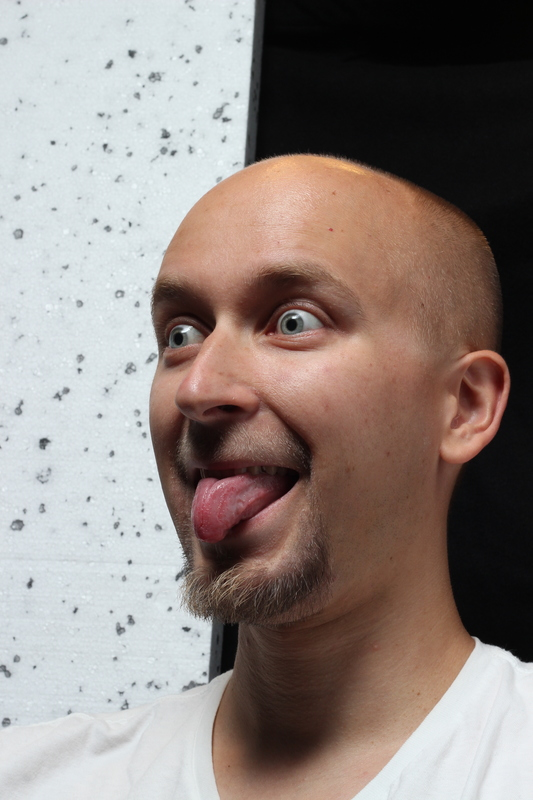
\includegraphics[width=0.3\textwidth]{arto-1}
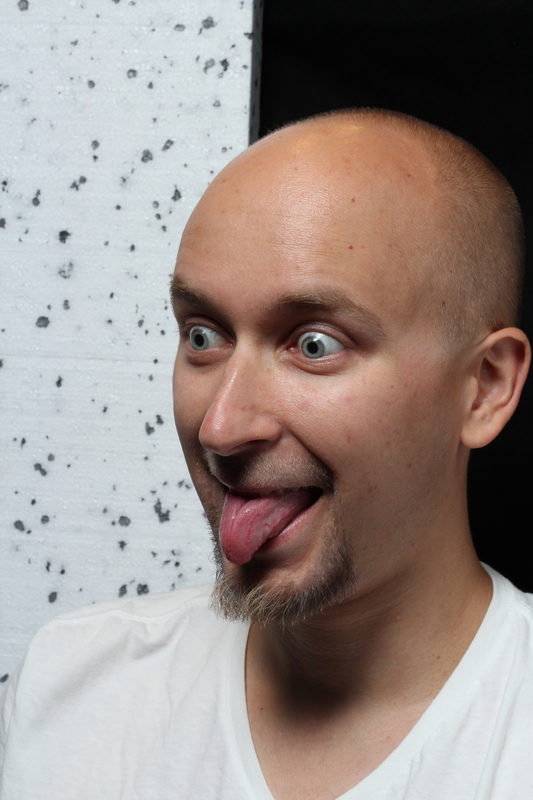
\includegraphics[width=0.3\textwidth]{arto-2}
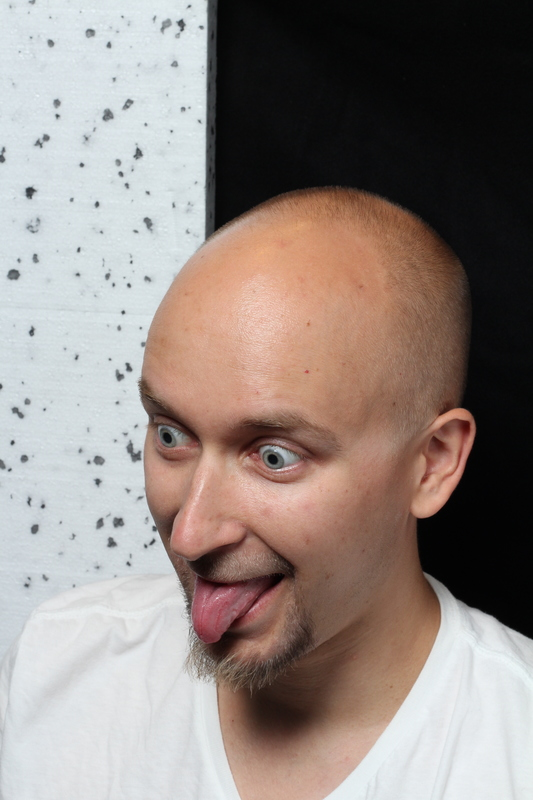
\includegraphics[width=0.3\textwidth]{arto-3}
}{fig:sample-arto-photoscan}{
	Three of the nine source pictures for a head scan
}

\simplefig{h}{%
%\includegraphics[width=0.4\textwidth]{photoscan-arto-sparse}
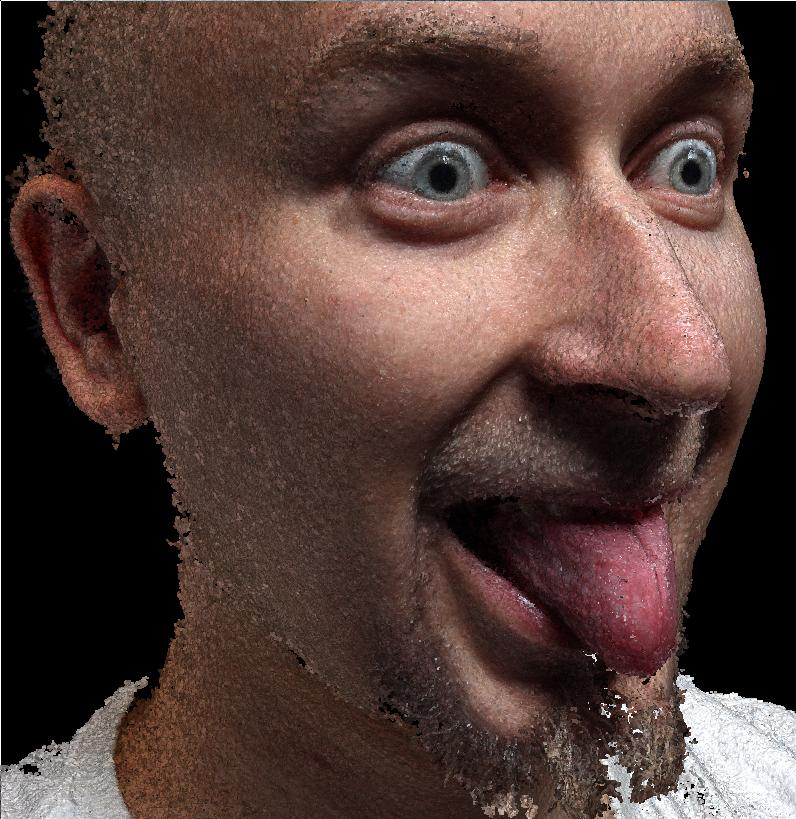
\includegraphics[width=0.35\textwidth]{photoscan-arto-dense}
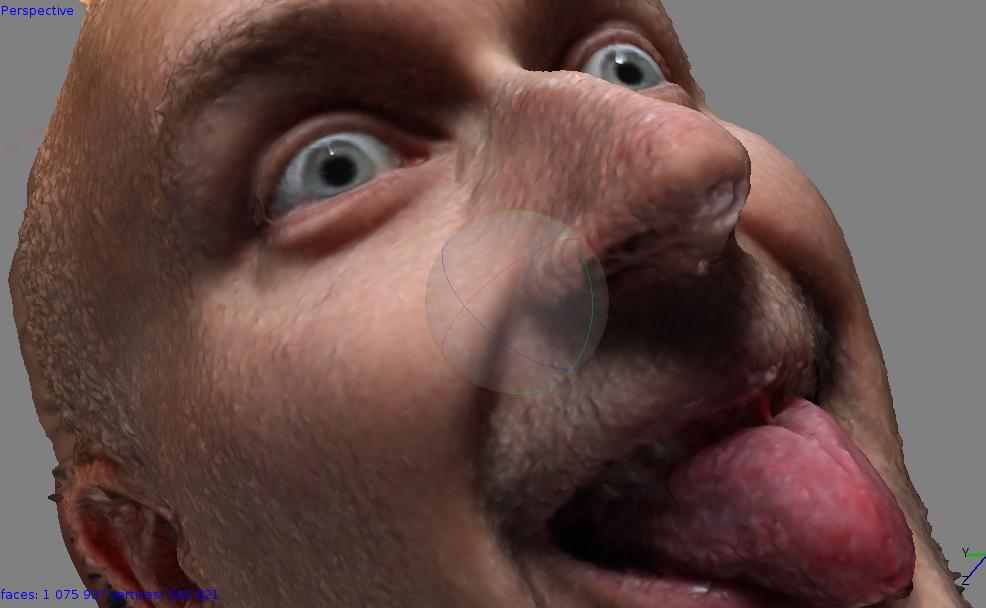
\includegraphics[width=0.4\textwidth]{photoscan-arto-textured}
}{fig:sample-arto-photoscan}{
	Arto in Photoscan
}

\simplefig{h}{%
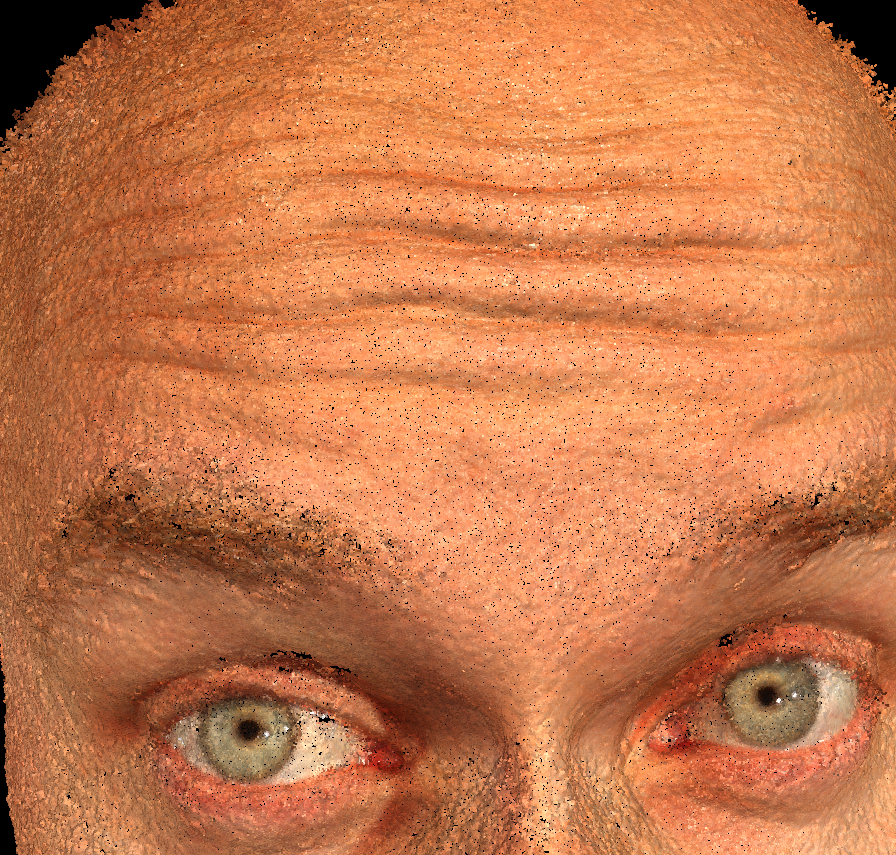
\includegraphics[width=0.48\textwidth]{arto-forehead-dense}%
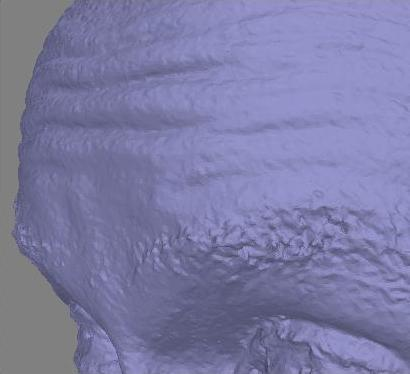
\includegraphics[width=0.48\textwidth]{arto-forehead-solid}\\%
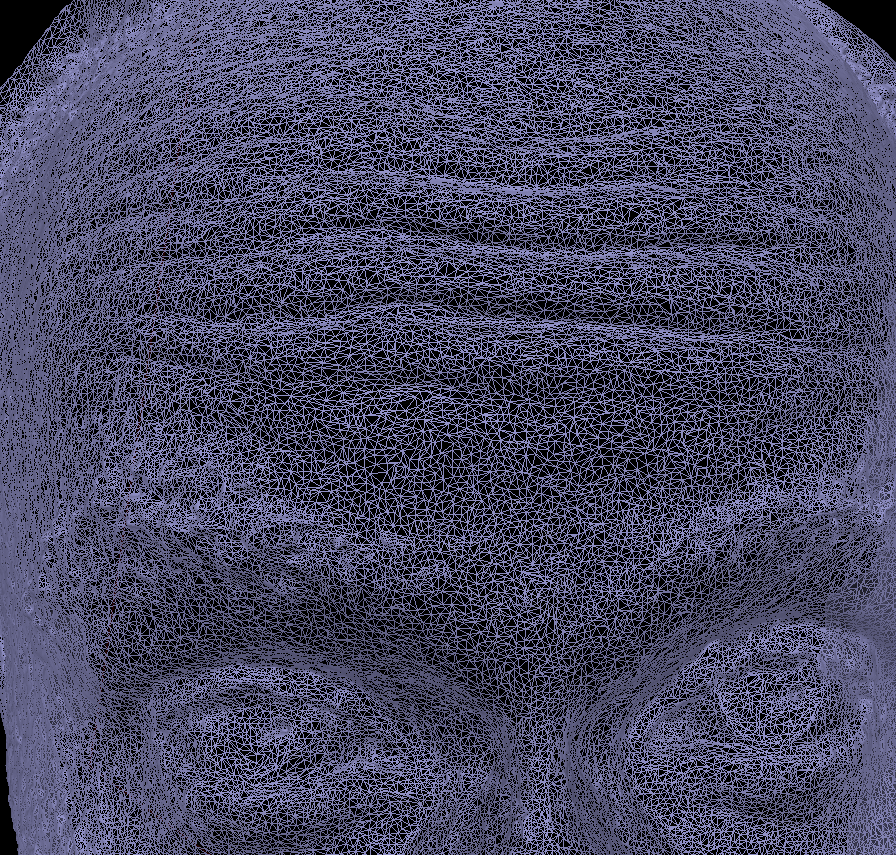
\includegraphics[width=0.48\textwidth]{arto-forehead-wireframe}%
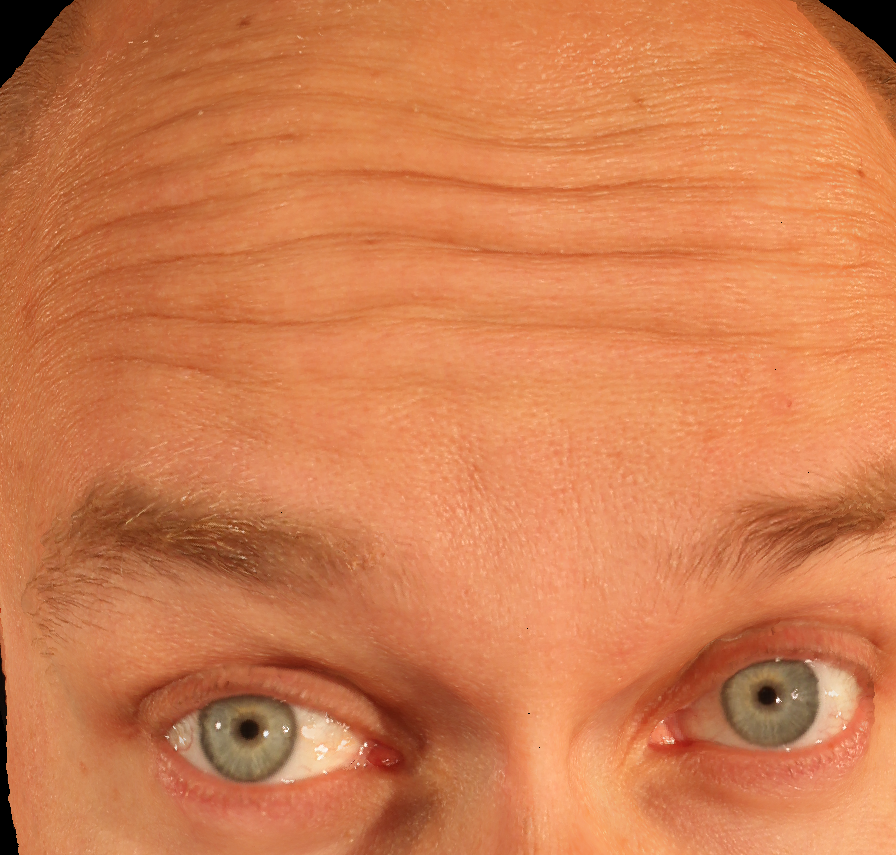
\includegraphics[width=0.48\textwidth]{arto-forehead-tex}\\%
}{fig:sample-arto-forehead}{
	Forehead wrinkles in PhotoScan: dense point cloud, solid mesh, wireframe, and textured mesh.
	The point cloud and wireframe pictures show the reconstructed detail level well.
}

\simplegfx{h}{\textwidth}{arto-forehead-uvmap}{
	UV map for the model in figure \ref{fig:sample-arto-forehead}. Note the wrinkle colors in the forehead patches.
}


VisualSFM \cite{visualsfm} is a free SfM system combining the initial steps of structure reconstruction, and has integration for dense reconstruction using the PMVS \cite{pmvs} tool and others.
Same datasets were tested as with Photoscan with similar results.
VisualSFM's feature matching seems not as robust, sometimes resulting in separate models.
PMVS \cite{pmvs} works by expanding patches in the reconstruction, resulting in a dense point cloud with oriented and colored points.
For mesh generation, the result was imported into \cite{Meshlab}.
The outlier points were cleaned up manually, and a mesh was fitted using the Poisson surface reconstruction plugin.
Results of different steps of the pipeline can be seen in figure \ref{fig:sample-arto-meshlab}.

%\simplefig{h}{%
%%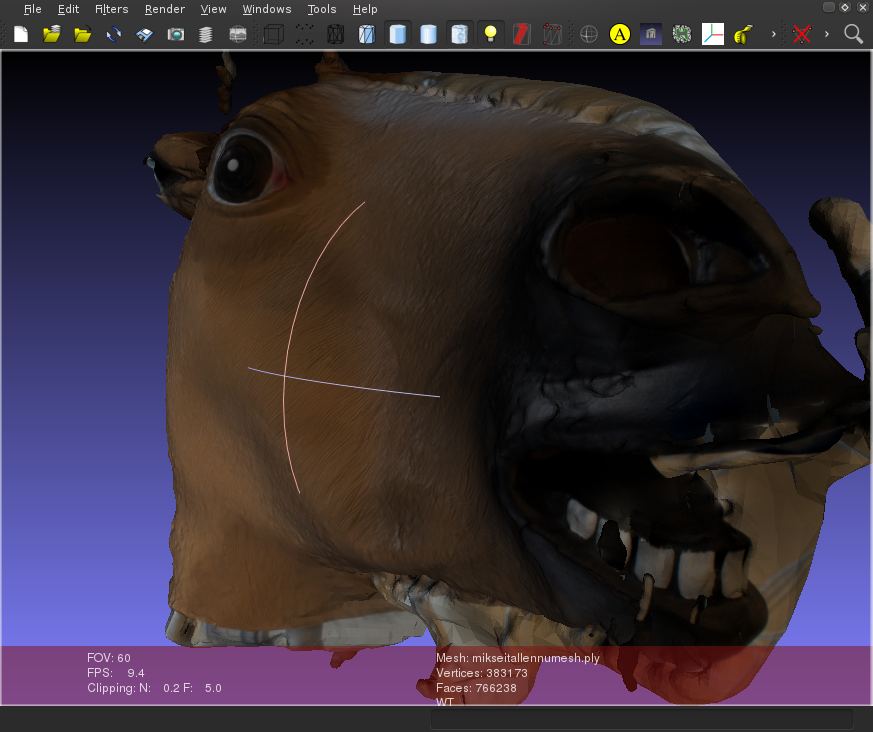
\includegraphics[width=0.4\textwidth]{meshlab}
%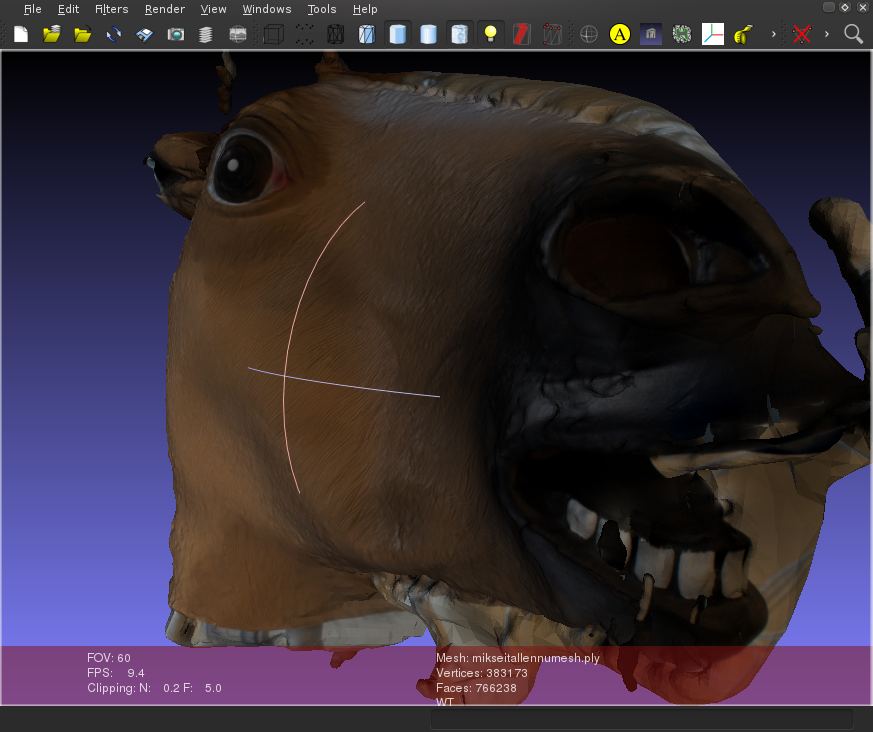
\includegraphics[width=0.4\textwidth]{meshlab}
%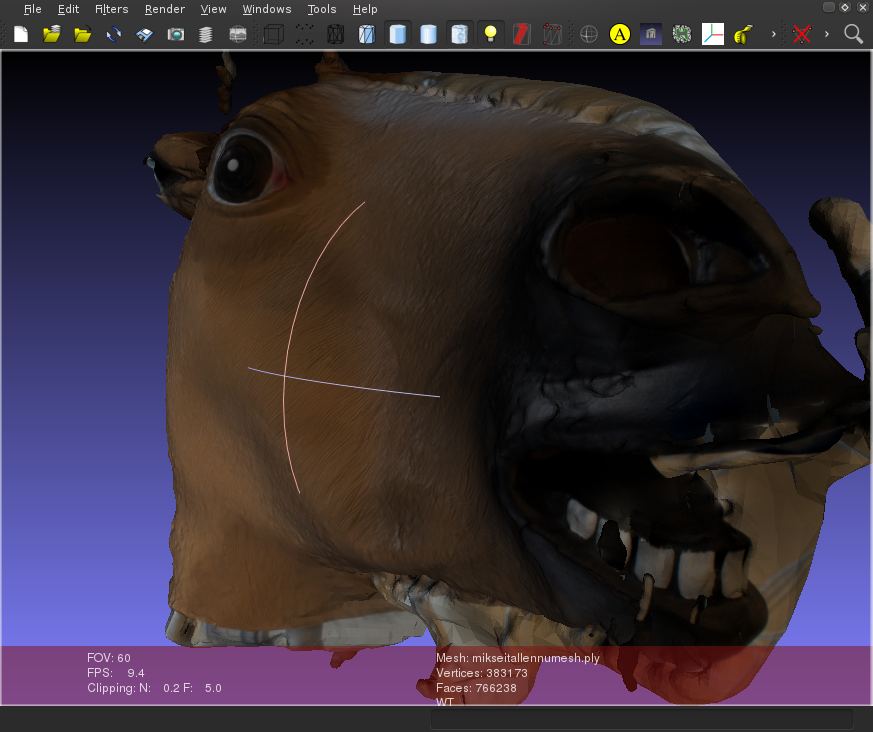
\includegraphics[width=0.4\textwidth]{meshlab}
%}{fig:sample-arto}{
%	Arto in Photoscan
%}

A structure of Lego blocks was scanned with poor results, as was expected; uniform-colored blocks with no texture and no geometry variations present a difficulty to point matching.

%\simplegfx{h!}{\textwidth}{legoshit}{
%	lego
%}

\subsection{Hard cases}

Low light? Little texture? Speculars? Hair?

% test X. not feasible for X because Y.

\subsection{Accuracy}

\clearpage

\section{Discussion}

%Perf of cloth animation capture

%other uses - street view, autom driving, geodetic systems

%(corresponding problems in e.g. autonomous driving or harvester machines?)

%(any point in outdoor methods?)


%previous usage in:
%
%	rockstar games / la noire; camera pairs
%
%	polar express / sony imageworks
%
%	ea sports / faro



\subsection{Feasibility}

\subsection{Facial surface motion capture} % {{{

\subsubsection{Deforming skin}

Surface capture of human skin is different from objects that consist of just connected rigid bodies: it stretches and shears in a highly non-predicatable way such that both its local geometry and texture changes, affected by the sub-surface properties of muscles etc.
Traditional methods for tracking rigid objects are thus not viable for high quality.
Joint motion capture has the rigid body assumption.

The deformations can be taken into account with e.g. furukawa etc.

Uncanny valley: humans are really good at identifying faces and correct facial movements; incorrect cases look really wrong.

\subsubsection{Simplifications/assumptions}

Facial expression space, 2d tracking, feature keypoints

Makeup

Facial expression space. Some techiques \cite{faceshift,something} use pre-recorded facial expressions to identify the subject's pose.
They suffer from not being able to accurately describe the temporal changes in finest details, but benefit from densely packed parameterization of facial expressions.
A separate mesh is stored as a three-dimensional template for each expression (such as happy or angry) and each frame is encoded, as a linear combination of these individual expressions.
%Such feature vectors describe well each possible face, and importantly, they eliminate the need for encoding the movement of each vertex, which can be unnecessarily heavy to compute or store.
%The results from this method can easily be mapped to other models than the face of the subject, as it is independent on the actual facial geometry and only uses weights for pre-modeled faces, making it interesting in computer animation.
%
Compare to Facial Action Coding System (FACS) (Hjortsjö 1969), which parameterizes the face in a group of muscular actions. This is similar to grouping vertices in keyframe animation [?].
%
%Expression tracking / 2d capture
%
%Use colors and highpass them; assume uniform lighting and locally uniform texture color (bradley).

\subsection{Future work}

%Although 

Constructing a 3D scanning rig was a large topic on its own.
The field of 3D reconstruction needs content to evolve, even more so for content-specific improvements.
The rig can be used for digitizing real-life objects and studying the process, helping to understand how different algorithms behave on different inputs.
Also, identifying defects in current state-of-the-art is easier when high-resolution test data can be scanned for testing new hypotheses.
%Although readily available multi-view datasets could be used for performance evaluation, not many sets are publicly available.
%the Stanford 3D Scanning Repository (models only)


volumetric reconstruction

octtree storage

octomap

space carving (photo-consistent shapes)

hole filling

visual hull

masking

Mesoscopic level shape reconstruction with texture (bradley)

match moving
